%%%%%%%%%%%%%%%%%%%%%%%%%%%%%%%%%%%%%%%%%
% Beamer Presentation
% LaTeX Template
% Version 1.0 (10/11/12)
%
% This template has been downloaded from:
% http://www.LaTeXTemplates.com
%
% License:
% CC BY-NC-SA 3.0 (http://creativecommons.org/licenses/by-nc-sa/3.0/)
%
%%%%%%%%%%%%%%%%%%%%%%%%%%%%%%%%%%%%%%%%%

%----------------------------------------------------------------------------------------
%	PACKAGES AND THEMES
%----------------------------------------------------------------------------------------

\documentclass{beamer}

\mode<presentation> {

% The Beamer class comes with a number of default slide themes
% which change the colors and layouts of slides. Below this is a list
% of all the themes, uncomment each in turn to see what they look like.

%\usetheme{default}
%\usetheme{AnnArbor}
%\usetheme{Antibes}
%\usetheme{Bergen}
%\usetheme{Berkeley}
%\usetheme{Berlin}
%\usetheme{Boadilla}
\usetheme{CambridgeUS}
%\usetheme{Copenhagen}
%\usetheme{Darmstadt}
%\usetheme{Dresden}
%\usetheme{Frankfurt}
%\usetheme{Goettingen}
%\usetheme{Hannover}
%\usetheme{Ilmenau}
%\usetheme{JuanLesPins}
%\usetheme{Luebeck}
%\usetheme{Madrid}
%\usetheme{Malmoe}
%\usetheme{Marburg}
%\usetheme{Montpellier}
%\usetheme{PaloAlto}
%\usetheme{Pittsburgh}
%\usetheme{Rochester}
%\usetheme{Singapore}
%\usetheme{Szeged}
%\usetheme{Warsaw}

% As well as themes, the Beamer class has a number of color themes
% for any slide theme. Uncomment each of these in turn to see how it
% changes the colors of your current slide theme.

%\usecolortheme{albatross}
%\usecolortheme{beaver}
%\usecolortheme{beetle}
%\usecolortheme{crane}
\usecolortheme{dolphin}
%\usecolortheme{dove}
%\usecolortheme{fly}
%\usecolortheme{lily}
%\usecolortheme{orchid}
%\usecolortheme{rose}
%\usecolortheme{seagull}
%\usecolortheme{seahorse}
%\usecolortheme{whale}
%\usecolortheme{wolverine}

%\setbeamertemplate{footline} % To remove the footer line in all slides uncomment this line
%\setbeamertemplate{footline}[page number] % To replace the footer line in all slides with a simple slide count uncomment this line

%\setbeamertemplate{navigation symbols}{} % To remove the navigation symbols from the bottom of all slides uncomment this line
}

\usepackage{graphicx} % Allows including images
\usepackage{booktabs} % Allows the use of \toprule, \midrule and \bottomrule in tables
\usepackage{mathrsfs}  
\usepackage{verbatim} 

%----------------------------------------------------------------------------------------
%	TITLE PAGE
%----------------------------------------------------------------------------------------

\title[VE216]{VE216 Recitation Class 5} % The short title appears at the bottom of every slide, the full title is only on the title page

\author{ZHU Yilun} % Your name
\institute[SJTU] % Your institution as it will appear on the bottom of every slide, may be shorthand to save space
{
UM-SJTU Joint Institute \\ % Your institution for the title page
\medskip
\textit{VE216 SU20 Teaching Group} % Your email address
}
\date{2020 Summer} % Date, can be changed to a custom date e.g.:\today

\begin{document}

\begin{frame}
\titlepage % Print the title page as the first slide
\end{frame}

\begin{frame}
\frametitle{Overview} % Table of contents slide, comment this block out to remove it
\tableofcontents % Throughout your presentation, if you choose to use \section{} and \subsection{} commands, these will automatically be printed on this slide as an overview of your presentation
\end{frame}

%----------------------------------------------------------------------------------------
%	PRESENTATION SLIDES
%----------------------------------------------------------------------------------------

%------------------------------------------------
\section{Chapter 3: Fourier Series}
%------------------------------------------------

\subsection{Properties}

\begin{frame}
   \frametitle{Properties} 
   \begin{itemize}
       \item Understand $ e^{j\theta}$
       \item Time shift: \[ x(t-t_0) \longleftrightarrow c_k e^{-jk\omega_0 t_0}  \]
       \item Differentiation: \[ y(t) = \frac{d}{dt} x(t) \longleftrightarrow jk\omega_0 c_k \]
       \item Etc ...
   \end{itemize}
\end{frame}

\subsection{Common FS Pairs}

\begin{frame}
    \frametitle{Common FS Pairs}
    \begin{figure}
        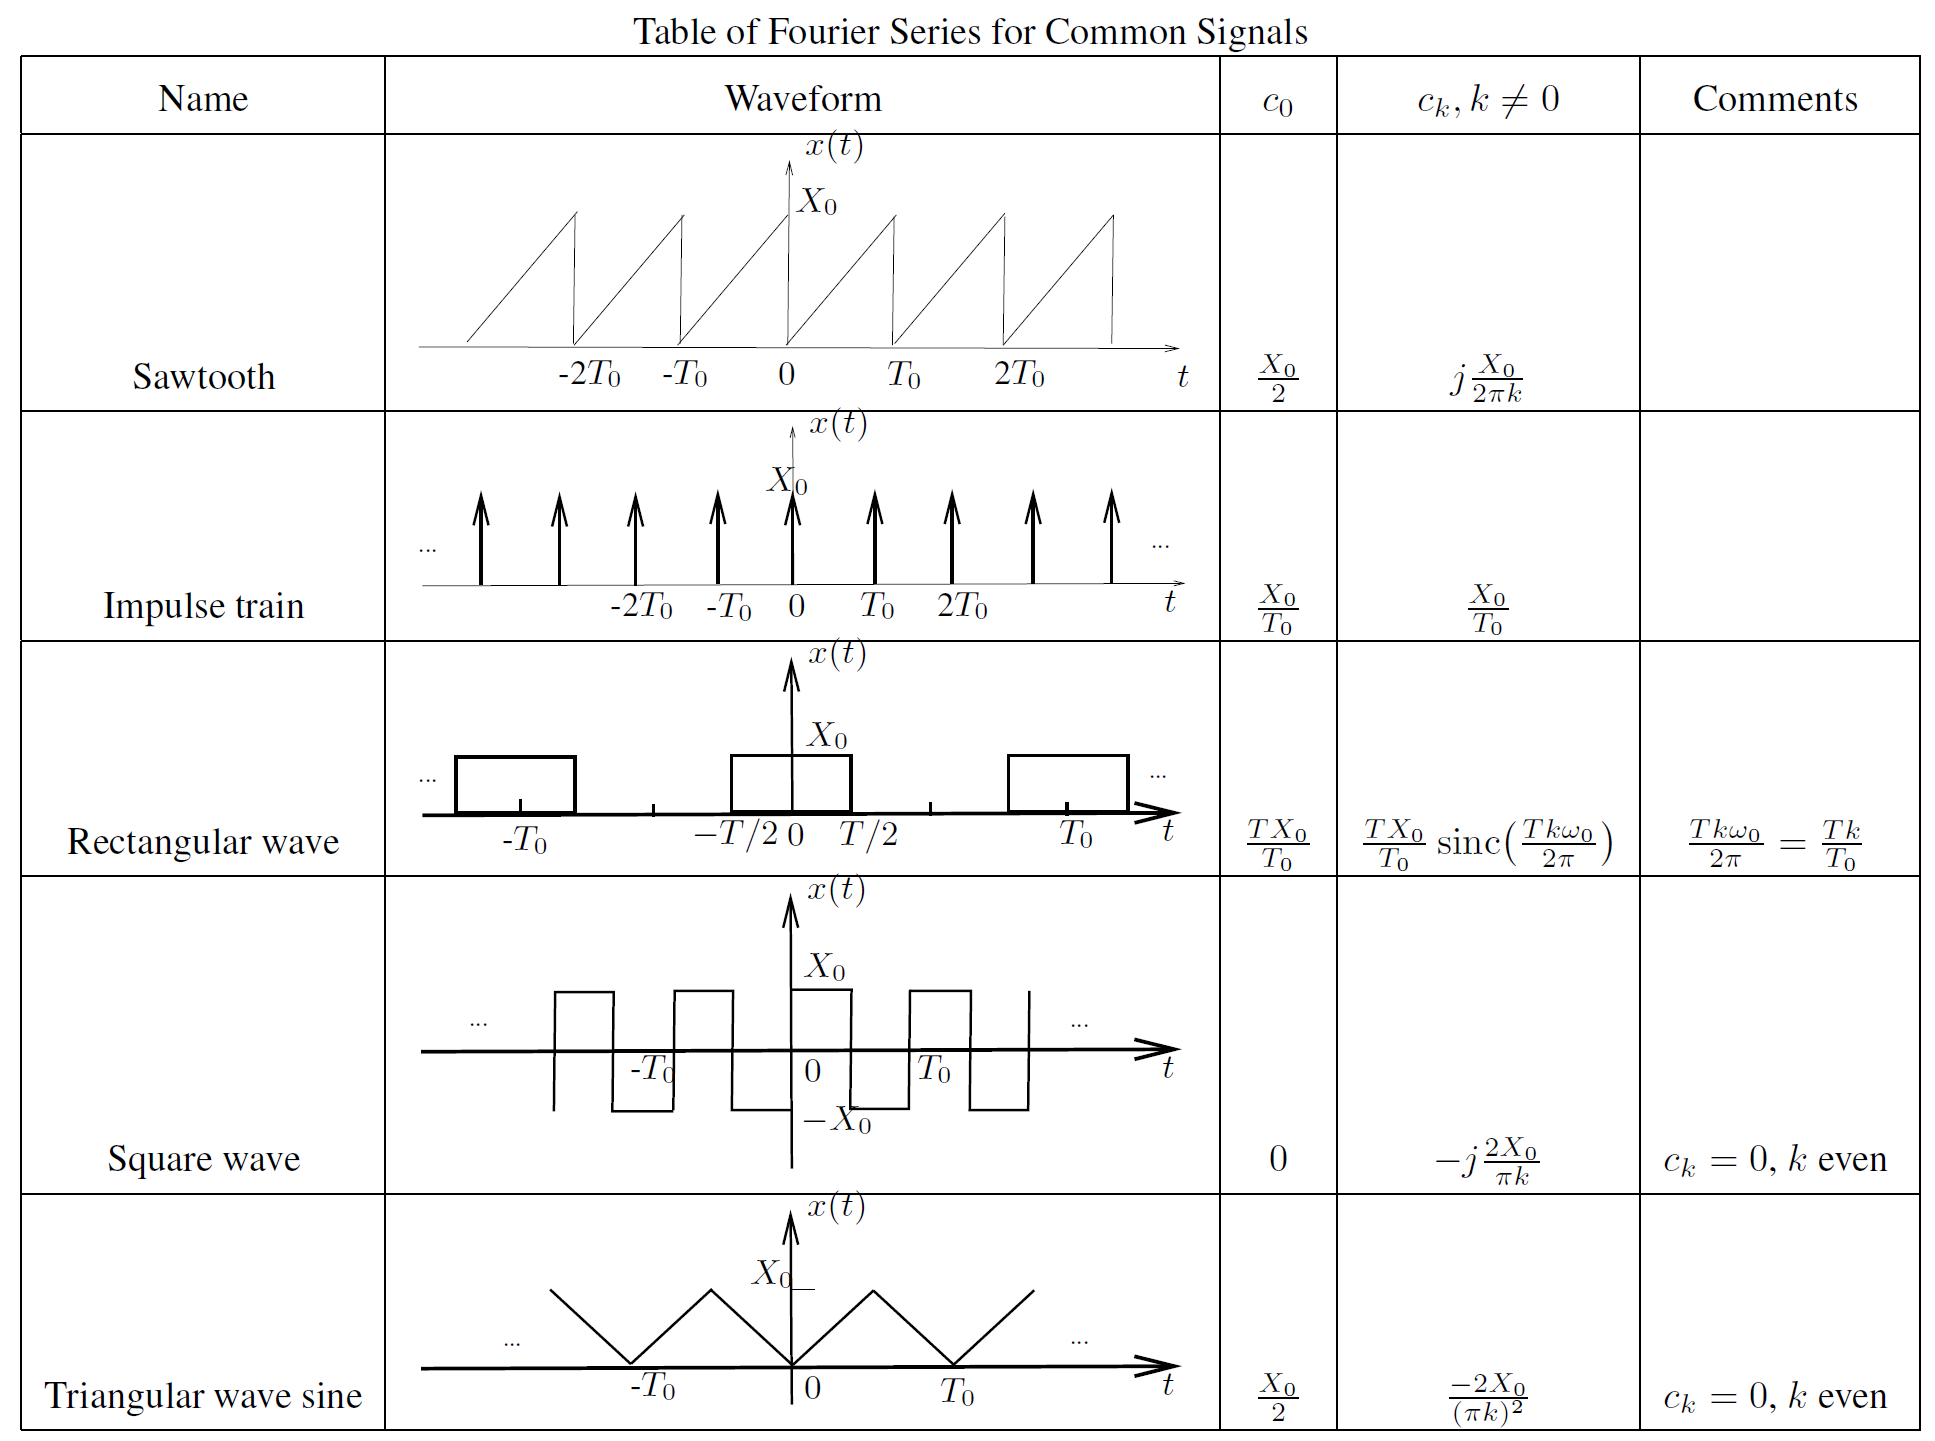
\includegraphics[width=0.8\linewidth]{FS_Table}
    \end{figure}
\end{frame}

\begin{frame}[t]
    \frametitle{To help remember}
    \begin{figure}
        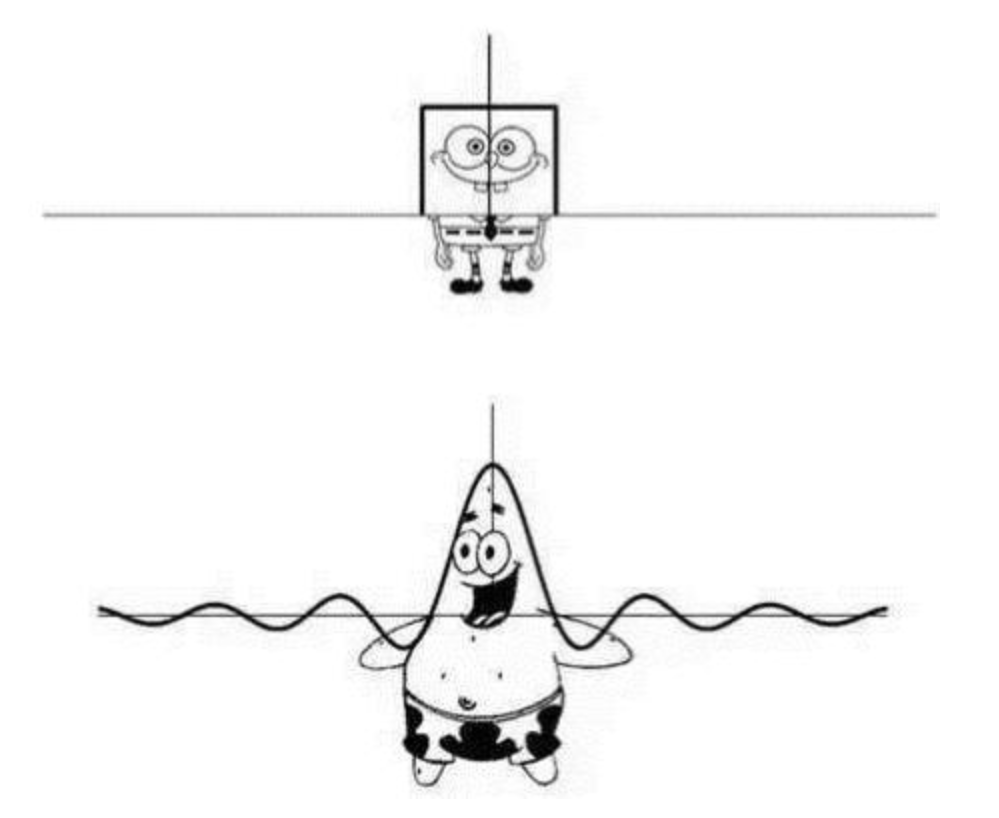
\includegraphics[width=0.4\linewidth]{sponge.PNG}
    \end{figure}
    \begin{center}
        \begin{align*}
            \text{SpongeBob SquarePants} &\stackrel{FT}{\longleftrightarrow}  \text{Patrick Star} \\[1em]
            \text{Periodic SpongeBob SquarePants} &\stackrel{FS}{\longleftrightarrow}  \text{Samples of Patrick Star} \\[1em]            
        \end{align*}
    \end{center} 
\end{frame}

\begin{frame}[t]
    \frametitle{Exercise - Use Table Lookup: Quiz3}
    \begin{figure}
        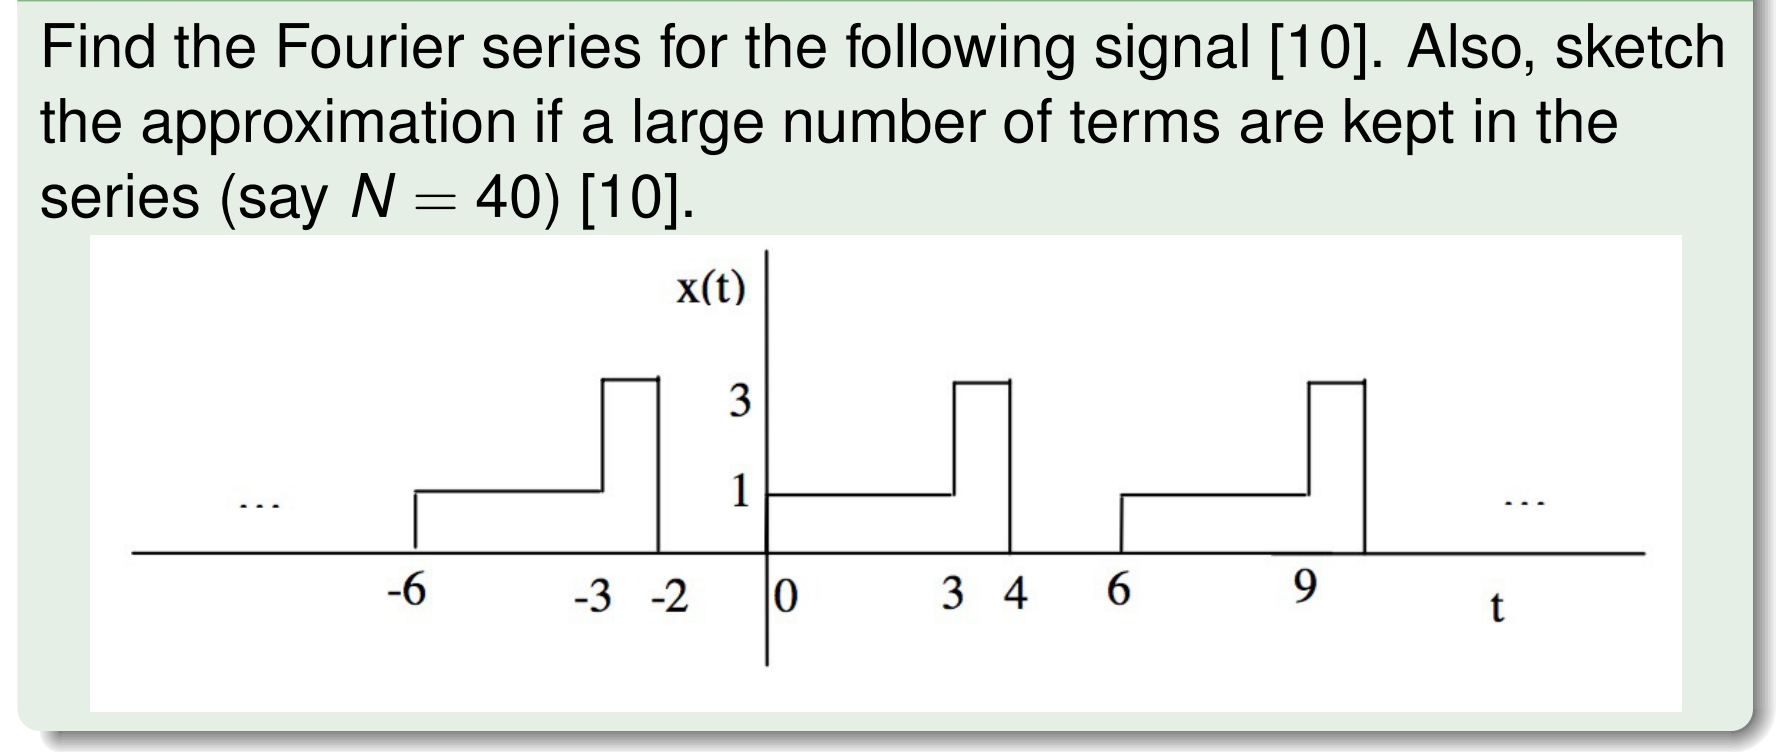
\includegraphics[width=0.7\linewidth]{quiz3.PNG}
    \end{figure}
\end{frame}


%------------------------------------------------
\section{Chapter 4: Fourier Transform}
%------------------------------------------------

\subsection{FS vs FT}

\begin{frame}
    \frametitle{FS vs FT: definition}
    Fourier Series: for periodic signals
    \begin{figure}
        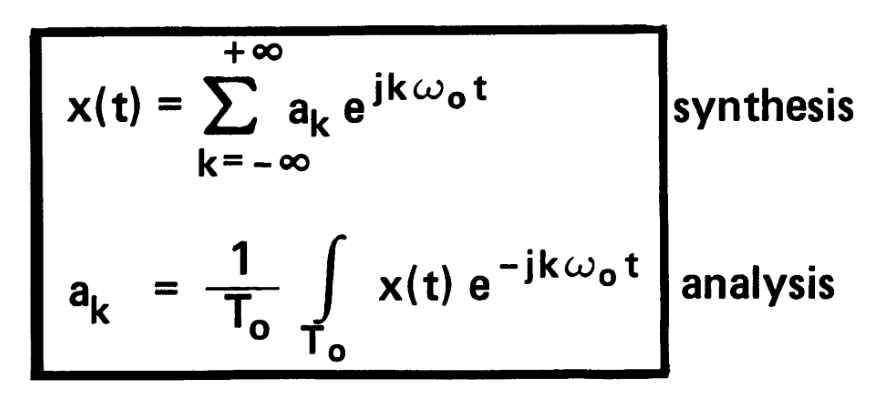
\includegraphics[width=0.4\linewidth]{FS_def}
    \end{figure}
    Fourier Transform: for ``all'' signals, often aperiodic
    \begin{figure}
        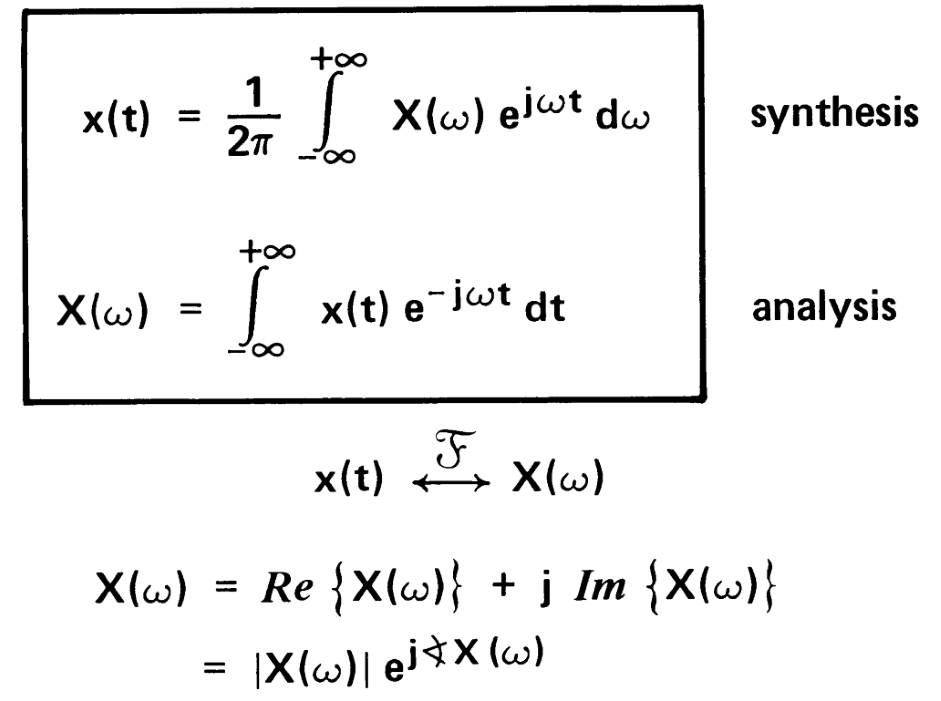
\includegraphics[width=0.4\linewidth]{FT_def}
    \end{figure}
\end{frame}


\begin{frame}
    \frametitle{FS vs FT: for periodic signal}
    \begin{figure}
        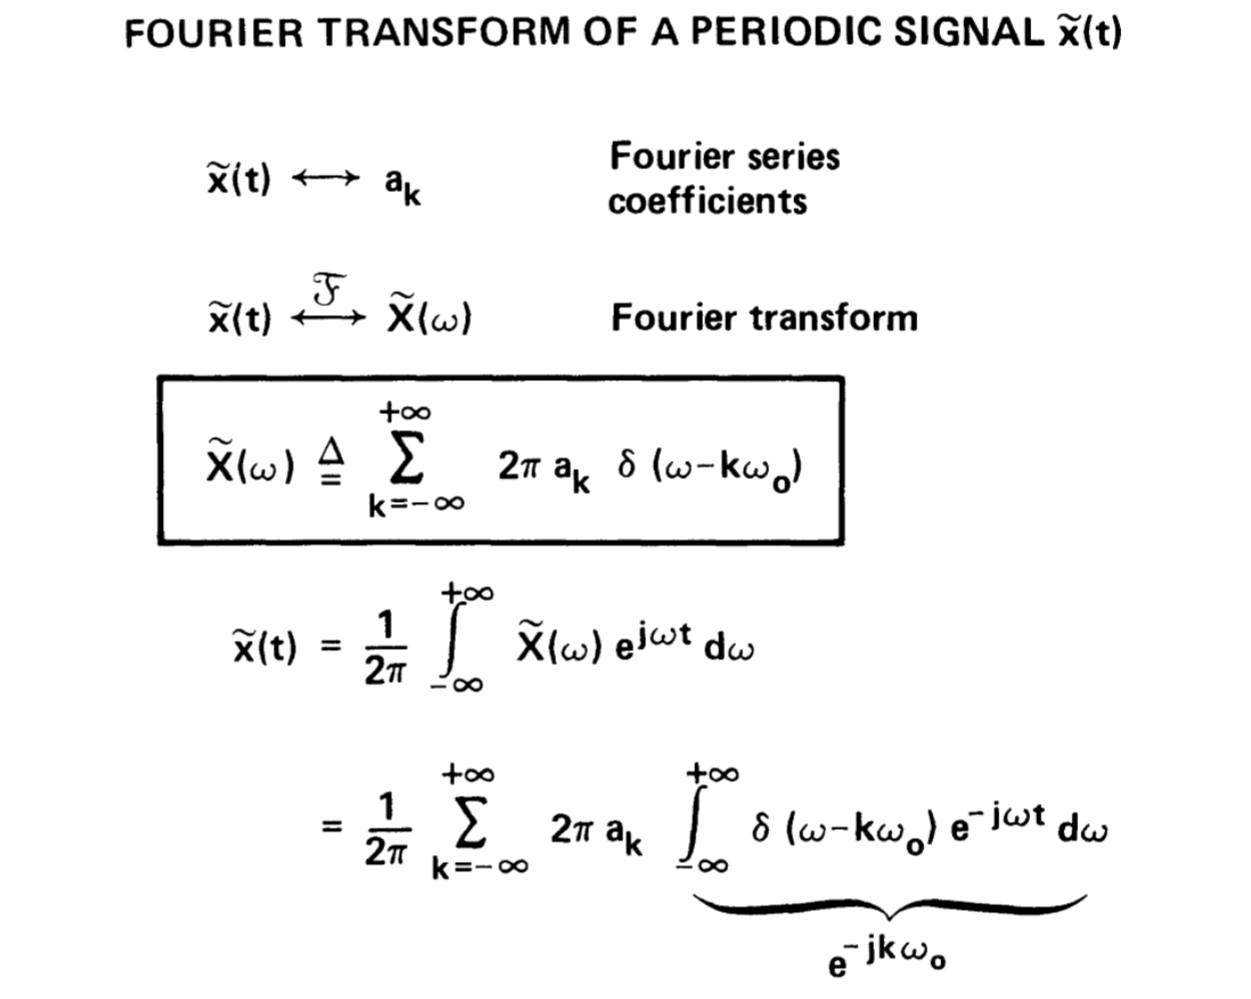
\includegraphics[width=0.7\linewidth]{FSvsFT}
    \end{figure}
\end{frame}

\begin{frame}
    \frametitle{FS vs FT: for periodic signal - Example}
    \begin{figure}
        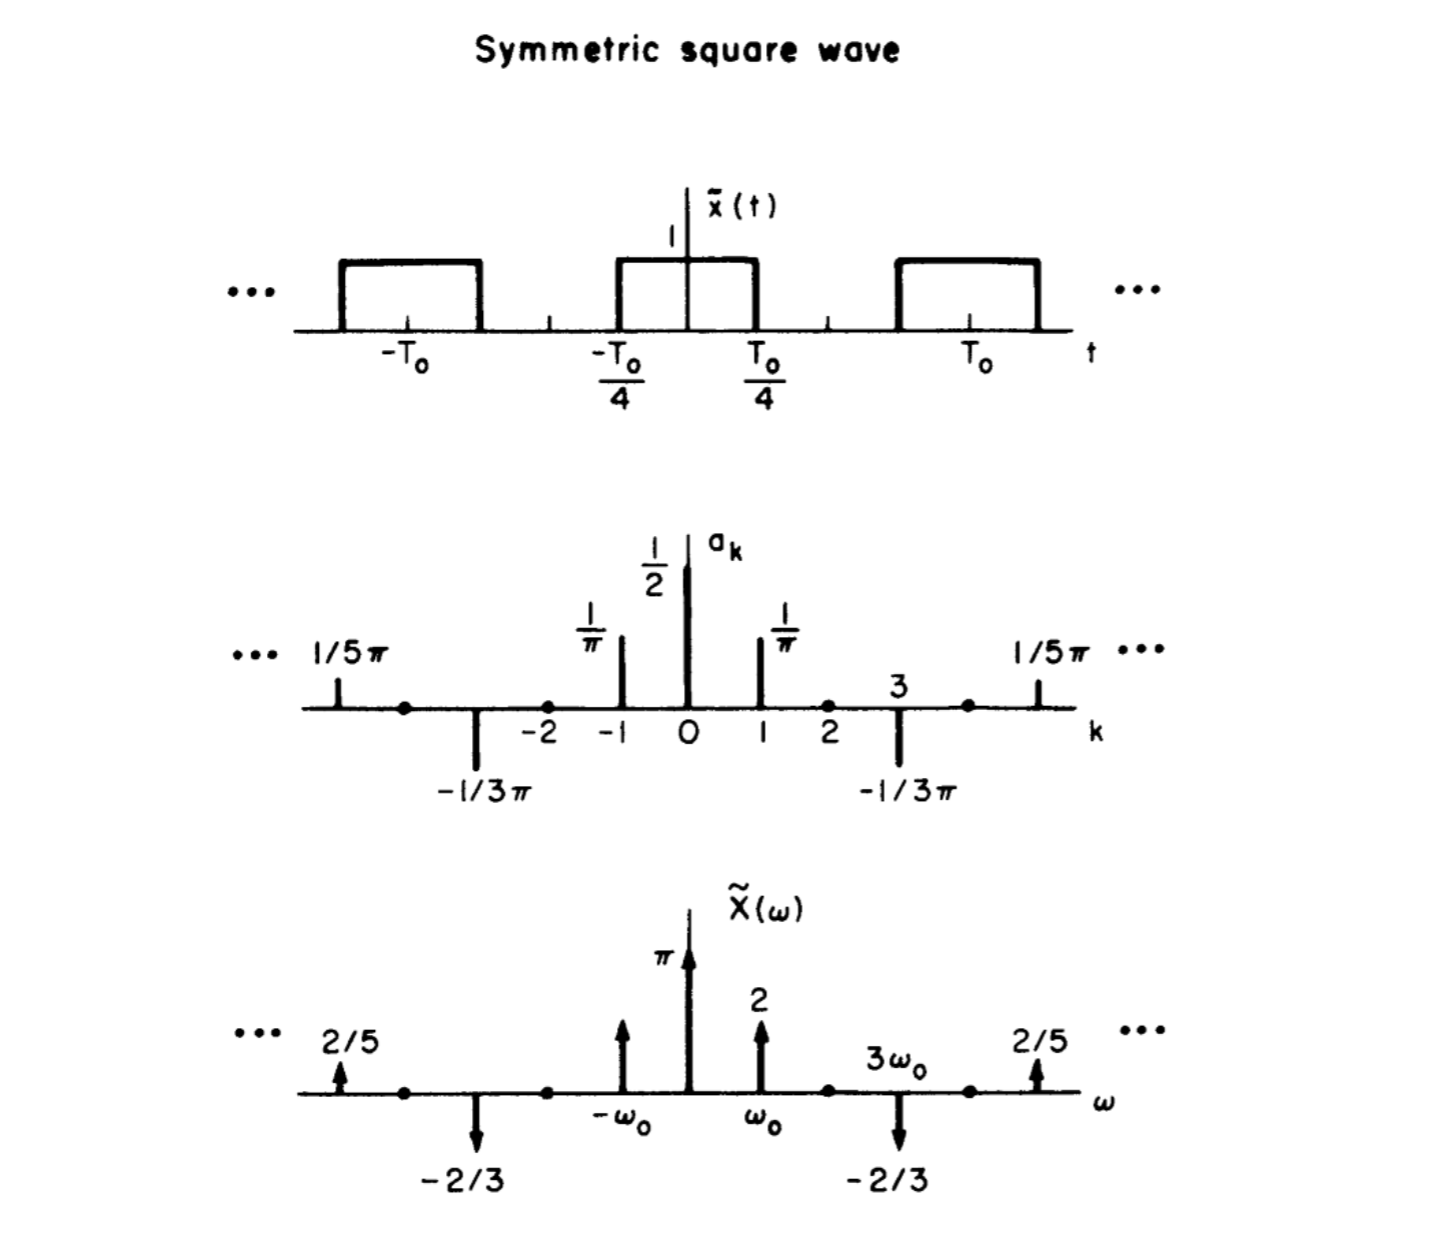
\includegraphics[width=0.7\linewidth]{FSvsFT_eg}
    \end{figure}
\end{frame}

\begin{frame}[t]
    \frametitle{FS vs FT: for periodic signal - Quiz4 Q1}
    \begin{figure}
        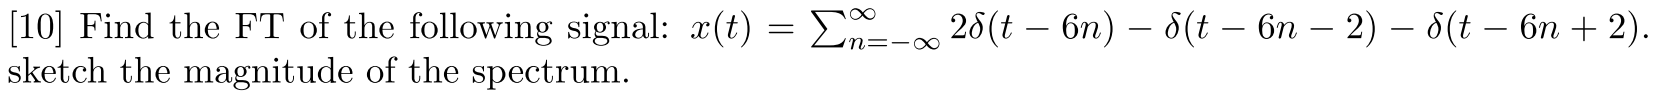
\includegraphics[width=1\linewidth]{quiz4q1.png}
    \end{figure}

\end{frame}

\subsection{Common FT Pairs}
\begin{frame}
    \frametitle{Common FT Pairs}
\begin{center}
    \begin{align*}
        \delta(t) &\stackrel{\mathscr{F}}{\longleftrightarrow}  1 \\[1em]
        \delta(t-t_0) &\stackrel{\mathscr{F}}{\longleftrightarrow}  e^{-jk\omega t_0} \\[1em]
        1 &\stackrel{\mathscr{F}}{\longleftrightarrow}  2\pi \delta(\omega) \\[1em]
        e^{j\omega_0 t} &\stackrel{\mathscr{F}}{\longleftrightarrow} 2 \pi \delta(\omega - \omega_0) \\[1em]
        \cos(\omega_0 t) &\stackrel{\mathscr{F}}{\longleftrightarrow} \pi \delta(\omega - \omega_0) + \pi \delta(\omega + \omega_0)
    \end{align*}
\end{center} 

\end{frame}


\subsection{Properties}


\begin{frame}
   \frametitle{Properties} 
   \begin{itemize}       
       \item Time shift: \[ f(t - \tau) \stackrel{\mathscr{F}}{\longleftrightarrow} F(\omega) e^{-j \omega \tau}   \]
       \item Time reversal: \[ f(-t) \stackrel{\mathscr{F}}{\longleftrightarrow} F(-\omega)
           \]
       \item Time Differentiation: \[ \frac{d^n}{dt^n} f(t) \stackrel{\mathscr{F}}{\longleftrightarrow} (j\omega)^n F(\omega)
           \]
        \item Freq. Differentiation: \[ (-jt)^nf(t) \stackrel{\mathscr{F}}{\longleftrightarrow} \frac{d^n}{d\omega^n} F(\omega)
            \] 
        \item Hermitian: If f(t) real, then \[  F(-\omega) = F^*(\omega) \]
   \end{itemize}
\end{frame}

\begin{frame}[t]
    \frametitle{Exercise - Use FT Table}
    \begin{block}{HW4 Q3}
        Find the FT of $t^2 e^{-(t/2)^2}$
    \end{block}
    Hint: 
    \begin{itemize}
        \item $ e^{-bt^2} \stackrel{\mathscr{F}}{\longleftrightarrow} \sqrt{\pi/b} e^{-\omega^2/4b}  $ 
        \item $ (-jt)^nf(t) \stackrel{\mathscr{F}}{\longleftrightarrow} \frac{d^n}{d\omega^n} F(\omega) $
    \end{itemize}

\end{frame}

\section{Summary}
\begin{frame}
    \frametitle{Summary}
    \begin{itemize}
        \item FS vs FT
        \item FS Table, FT Table
        \item Next week: 
        \begin{itemize}
            \item Closure of FT
            \item Focus on Filtering (problem-solving)
        \end{itemize}
        \item The place we are in the big picture
        \item Actually, we will spend a whole month on the applications related to FS and FT
    \end{itemize}
\end{frame}

%------------------------------------------------

\begin{frame}
\Huge{\centerline{The End}}
\end{frame}

%----------------------------------------------------------------------------------------

\end{document} 